%% 由 build/emit_tex.py 生成（生成物，勿手改）；定制请放 user_style.tex / user_meta.yaml
\chapter{Sympy及其基本使用}\label{sympyux53caux5176ux57faux672cux4f7fux7528}

\section{01
符号对象与基本运算：创建、算术、极限、微分与积分}\label{ux7b26ux53f7ux5bf9ux8c61ux4e0eux57faux672cux8fd0ux7b97ux521bux5efaux7b97ux672fux6781ux9650ux5faeux5206ux4e0eux79efux5206}

\begin{quote}
本节对应原版 2.1 的内容，并增补学习目标、常见误区、思考题与延伸阅读。
所有代码输出均为实际运行结果（SymPy 1.13.1）。
\end{quote}

\subsection{本节目标}\label{ux672cux8282ux76eeux6807-11}

\begin{itemize}
\tightlist
\item
  理解``符号对象（symbolic object）''与``数值对象''的区别；
\item
  会用 \texttt{symbols} / \texttt{Symbol} 创建符号，并设置
  \texttt{positive}、\texttt{real}、\texttt{integer} 等假设；
\item
  掌握符号的四则运算、常用数学函数（\texttt{sin}、\texttt{cos}、\texttt{exp}
  等）；
\item
  会求极限（\texttt{limit}）、导数/偏导数（\texttt{diff}）、不定积分与定积分（\texttt{integrate}）；
\item
  会用
  \texttt{simplify}、\texttt{factor}、\texttt{expand}、\texttt{trigsimp}
  化简，用 \texttt{subs} / \texttt{evalf} / \texttt{N} 做替换与数值化；
\item
  了解 \texttt{series}（级数展开）等进阶工具。
\end{itemize}

\subsection{先修}\label{ux5148ux4fee-4}

\begin{itemize}
\tightlist
\item
  Python 变量、函数、字符串；
\item
  微积分中的极限、导数、积分概念（不要求会手算复杂积分）。
\end{itemize}

\subsection{官方文档/参考入口}\label{ux5b98ux65b9ux6587ux6863ux53c2ux8003ux5165ux53e3}

\begin{itemize}
\tightlist
\item
  SymPy 官方
  Tutorial（符号、化简、微积分）：https://docs.sympy.org/latest/tutorials/index.html
\item
  SymPy 官方
  Calculus：https://docs.sympy.org/latest/tutorials/intro-tutorial/calculus.html
\end{itemize}

\begin{center}\rule{0.5\linewidth}{0.5pt}\end{center}

\subsection{1.1 为什么用 SymPy}\label{ux4e3aux4ec0ux4e48ux7528-sympy}

NumPy 擅长\textbf{数值}计算：把数字代入后算出一个近似值。SymPy
则进行\textbf{符号}计算：把 \(x\)、\(y\) 当作字母，推导出精确表达式。

{\def\LTcaptype{none} % do not increment counter
\begin{longtable}[]{@{}lll@{}}
\toprule\noalign{}
特性 & NumPy（数值） & SymPy（符号） \\
\midrule\noalign{}
\endhead
\bottomrule\noalign{}
\endlastfoot
代表对象 & \texttt{ndarray} & \texttt{Symbol} / \texttt{Expr} \\
\(\int_0^1 x^2\,dx\) & 返回 0.3333333333 & 返回精确的 \(1/3\) \\
解方程 & 数值迭代 & 精确根 \(\sqrt{2}\) 等 \\
用途 & 大规模数值模拟 & 公式推导、理论验证 \\
\end{longtable}
}

实际工作中二者常配合使用：先用 SymPy 推导出公式，再 \texttt{lambdify}
成数值函数（见 02 节）交给 NumPy 计算。

\subsection{1.2
符号对象的创建}\label{ux7b26ux53f7ux5bf9ux8c61ux7684ux521bux5efa}

\subsubsection{\texorpdfstring{1.2.1
一次创建多个符号：\texttt{symbols}}{1.2.1 一次创建多个符号：symbols}}\label{ux4e00ux6b21ux521bux5efaux591aux4e2aux7b26ux53f7symbols}

\begin{Shaded}
\begin{Highlighting}[]
\ImportTok{import}\NormalTok{ sympy }\ImportTok{as}\NormalTok{ sp}
\NormalTok{x, y, z }\OperatorTok{=}\NormalTok{ sp.symbols(}\StringTok{\textquotesingle{}x y z\textquotesingle{}}\NormalTok{)}
\BuiltInTok{print}\NormalTok{(x }\OperatorTok{+}\NormalTok{ y }\OperatorTok{+}\NormalTok{ z)}
\end{Highlighting}
\end{Shaded}

\begin{Shaded}
\begin{Highlighting}[]
\NormalTok{x + y + z}
\end{Highlighting}
\end{Shaded}

\subsubsection{\texorpdfstring{1.2.2
单个符号：\texttt{Symbol}}{1.2.2 单个符号：Symbol}}\label{ux5355ux4e2aux7b26ux53f7symbol}

\begin{Shaded}
\begin{Highlighting}[]
\NormalTok{x }\OperatorTok{=}\NormalTok{ sp.Symbol(}\StringTok{\textquotesingle{}x\textquotesingle{}}\NormalTok{)}
\BuiltInTok{print}\NormalTok{(x)}

\NormalTok{positive\_x }\OperatorTok{=}\NormalTok{ sp.Symbol(}\StringTok{\textquotesingle{}x\textquotesingle{}}\NormalTok{, positive}\OperatorTok{=}\VariableTok{True}\NormalTok{)}
\BuiltInTok{print}\NormalTok{(positive\_x)}
\end{Highlighting}
\end{Shaded}

\begin{Shaded}
\begin{Highlighting}[]
\NormalTok{x}
\NormalTok{x}
\end{Highlighting}
\end{Shaded}

\begin{quote}
\textbf{注意}：\texttt{positive=True} 并不改变打印结果，但会让 SymPy
在化简时利用``\(x>0\)''这个信息（例如 \(\sqrt{x^2}\) 会化简成 \(x\)）。
\end{quote}

其他常见假设：\texttt{real}（实数）、\texttt{integer}（整数）、\texttt{complex}（复数）。

\begin{Shaded}
\begin{Highlighting}[]
\NormalTok{real\_x }\OperatorTok{=}\NormalTok{ sp.Symbol(}\StringTok{\textquotesingle{}x\textquotesingle{}}\NormalTok{, real}\OperatorTok{=}\VariableTok{True}\NormalTok{)}
\NormalTok{integer\_n }\OperatorTok{=}\NormalTok{ sp.Symbol(}\StringTok{\textquotesingle{}n\textquotesingle{}}\NormalTok{, integer}\OperatorTok{=}\VariableTok{True}\NormalTok{)}
\BuiltInTok{print}\NormalTok{(real\_x)}
\BuiltInTok{print}\NormalTok{(integer\_n)}
\end{Highlighting}
\end{Shaded}

\begin{Shaded}
\begin{Highlighting}[]
\NormalTok{x}
\NormalTok{n}
\end{Highlighting}
\end{Shaded}

\subsubsection{1.2.3
创建一系列相关符号}\label{ux521bux5efaux4e00ux7cfbux5217ux76f8ux5173ux7b26ux53f7}

\begin{Shaded}
\begin{Highlighting}[]
\NormalTok{n }\OperatorTok{=} \DecValTok{3}
\NormalTok{xs }\OperatorTok{=}\NormalTok{ sp.symbols(}\SpecialStringTok{f\textquotesingle{}x\_1:}\SpecialCharTok{\{}\NormalTok{n}\OperatorTok{+}\DecValTok{1}\SpecialCharTok{\}}\SpecialStringTok{\textquotesingle{}}\NormalTok{)}
\BuiltInTok{print}\NormalTok{(xs)}

\NormalTok{x\_list }\OperatorTok{=}\NormalTok{ [sp.Symbol(}\SpecialStringTok{f\textquotesingle{}x\_}\SpecialCharTok{\{}\NormalTok{i}\OperatorTok{+}\DecValTok{1}\SpecialCharTok{\}}\SpecialStringTok{\textquotesingle{}}\NormalTok{) }\ControlFlowTok{for}\NormalTok{ i }\KeywordTok{in} \BuiltInTok{range}\NormalTok{(}\DecValTok{3}\NormalTok{)]}
\BuiltInTok{print}\NormalTok{(x\_list)}
\end{Highlighting}
\end{Shaded}

\begin{Shaded}
\begin{Highlighting}[]
\NormalTok{(x\_1, x\_2, x\_3)}
\NormalTok{[x\_1, x\_2, x\_3]}
\end{Highlighting}
\end{Shaded}

\subsection{1.3
符号对象的算术运算与常用函数}\label{ux7b26ux53f7ux5bf9ux8c61ux7684ux7b97ux672fux8fd0ux7b97ux4e0eux5e38ux7528ux51fdux6570}

\subsubsection{1.3.1 四则运算}\label{ux56dbux5219ux8fd0ux7b97-1}

\begin{Shaded}
\begin{Highlighting}[]
\NormalTok{x, y }\OperatorTok{=}\NormalTok{ sp.symbols(}\StringTok{\textquotesingle{}x y\textquotesingle{}}\NormalTok{)}
\BuiltInTok{print}\NormalTok{(x }\OperatorTok{+}\NormalTok{ y)}
\BuiltInTok{print}\NormalTok{(x }\OperatorTok{{-}}\NormalTok{ y)}
\BuiltInTok{print}\NormalTok{(x }\OperatorTok{*}\NormalTok{ y)}
\BuiltInTok{print}\NormalTok{(x }\OperatorTok{/}\NormalTok{ y)}
\end{Highlighting}
\end{Shaded}

\begin{Shaded}
\begin{Highlighting}[]
\NormalTok{x + y}
\NormalTok{x {-} y}
\NormalTok{x*y}
\NormalTok{x/y}
\end{Highlighting}
\end{Shaded}

\subsection{1.3.2 符号函数}\label{ux7b26ux53f7ux51fdux6570}

用 \texttt{Function} 可以定义``抽象函数''，但更常见的是直接使用 SymPy
预定义函数（\texttt{sin}、\texttt{cos}、\texttt{exp}、\texttt{log}、\texttt{sqrt}
等）。

\begin{Shaded}
\begin{Highlighting}[]
\NormalTok{x }\OperatorTok{=}\NormalTok{ sp.symbols(}\StringTok{\textquotesingle{}x\textquotesingle{}}\NormalTok{)}
\NormalTok{f }\OperatorTok{=}\NormalTok{ sp.Function(}\StringTok{\textquotesingle{}f\textquotesingle{}}\NormalTok{)(x)}
\BuiltInTok{print}\NormalTok{(f)}
\BuiltInTok{print}\NormalTok{(f.diff(x))          }\CommentTok{\# 抽象函数的导数}

\NormalTok{sin\_x }\OperatorTok{=}\NormalTok{ sp.sin(x)}
\NormalTok{cos\_x }\OperatorTok{=}\NormalTok{ sp.cos(x)}
\BuiltInTok{print}\NormalTok{(sin\_x)}
\BuiltInTok{print}\NormalTok{(cos\_x)}
\BuiltInTok{print}\NormalTok{(sin\_x }\OperatorTok{+}\NormalTok{ cos\_x)}
\end{Highlighting}
\end{Shaded}

\begin{Shaded}
\begin{Highlighting}[]
\NormalTok{f(x)}
\NormalTok{Derivative(f(x), x)}
\NormalTok{sin(x)}
\NormalTok{cos(x)}
\NormalTok{sin(x) + cos(x)}
\end{Highlighting}
\end{Shaded}

\subsection{1.4 极限运算}\label{ux6781ux9650ux8fd0ux7b97}

\texttt{limit(expression,\ variable,\ point,\ dir=\textquotesingle{}+\textquotesingle{})}
的四个参数分别是被求极限的表达式、变量、趋近点、方向（\texttt{\textquotesingle{}+\textquotesingle{}}
右极限、\texttt{\textquotesingle{}-\textquotesingle{}}
左极限、\texttt{\textquotesingle{}+-\textquotesingle{}}
双侧）。\texttt{oo} 表示无穷大。

\begin{Shaded}
\begin{Highlighting}[]
\NormalTok{x }\OperatorTok{=}\NormalTok{ sp.symbols(}\StringTok{\textquotesingle{}x\textquotesingle{}}\NormalTok{)}
\BuiltInTok{print}\NormalTok{(sp.limit(sp.sin(x)}\OperatorTok{/}\NormalTok{x, x, }\DecValTok{0}\NormalTok{))        }\CommentTok{\# 重要极限 {-}\textgreater{} 1}
\BuiltInTok{print}\NormalTok{(sp.limit(}\DecValTok{1}\OperatorTok{/}\NormalTok{x, x, sp.oo))            }\CommentTok{\# x 趋近 +oo {-}\textgreater{} 0}
\BuiltInTok{print}\NormalTok{(sp.limit(}\DecValTok{1}\OperatorTok{/}\NormalTok{x, x, }\DecValTok{0}\NormalTok{, }\BuiltInTok{dir}\OperatorTok{=}\StringTok{\textquotesingle{}{-}\textquotesingle{}}\NormalTok{))       }\CommentTok{\# 左极限 {-}\textgreater{} {-}oo}
\BuiltInTok{print}\NormalTok{(sp.limit(x}\OperatorTok{**}\DecValTok{3} \OperatorTok{+} \DecValTok{3}\OperatorTok{*}\NormalTok{x}\OperatorTok{**}\DecValTok{2} \OperatorTok{+}\NormalTok{ sp.exp(}\OperatorTok{{-}}\DecValTok{2}\OperatorTok{*}\NormalTok{x), x, }\FloatTok{0.5}\NormalTok{))}
\end{Highlighting}
\end{Shaded}

\begin{Shaded}
\begin{Highlighting}[]
\NormalTok{1}
\NormalTok{0}
\NormalTok{{-}oo}
\NormalTok{1.24287944117144}
\end{Highlighting}
\end{Shaded}

\subsection{1.5 微分运算}\label{ux5faeux5206ux8fd0ux7b97}

\subsubsection{1.5.1
一元函数求导}\label{ux4e00ux5143ux51fdux6570ux6c42ux5bfc}

\begin{Shaded}
\begin{Highlighting}[]
\NormalTok{x }\OperatorTok{=}\NormalTok{ sp.symbols(}\StringTok{\textquotesingle{}x\textquotesingle{}}\NormalTok{)}
\NormalTok{f }\OperatorTok{=}\NormalTok{ x}\OperatorTok{**}\DecValTok{2} \OperatorTok{+} \DecValTok{3}\OperatorTok{*}\NormalTok{x }\OperatorTok{+} \DecValTok{2}
\BuiltInTok{print}\NormalTok{(sp.diff(f, x))}

\NormalTok{g }\OperatorTok{=}\NormalTok{ sp.sin(x)}\OperatorTok{*}\NormalTok{sp.cos(x)}
\BuiltInTok{print}\NormalTok{(sp.diff(g, x))}
\BuiltInTok{print}\NormalTok{(sp.simplify(sp.diff(g, x)))        }\CommentTok{\# 化简为 cos(2x)}
\end{Highlighting}
\end{Shaded}

\begin{Shaded}
\begin{Highlighting}[]
\NormalTok{2*x + 3}
\NormalTok{{-}sin(x)**2 + cos(x)**2}
\NormalTok{cos(2*x)}
\end{Highlighting}
\end{Shaded}

\subsubsection{1.5.2
多元函数求偏导}\label{ux591aux5143ux51fdux6570ux6c42ux504fux5bfc}

\begin{Shaded}
\begin{Highlighting}[]
\NormalTok{x, y }\OperatorTok{=}\NormalTok{ sp.symbols(}\StringTok{\textquotesingle{}x y\textquotesingle{}}\NormalTok{)}
\NormalTok{h }\OperatorTok{=}\NormalTok{ x}\OperatorTok{**}\DecValTok{2} \OperatorTok{+}\NormalTok{ x}\OperatorTok{*}\NormalTok{y }\OperatorTok{+}\NormalTok{ y}\OperatorTok{**}\DecValTok{2}
\BuiltInTok{print}\NormalTok{(sp.diff(h, x))}
\BuiltInTok{print}\NormalTok{(sp.diff(h, y))}
\end{Highlighting}
\end{Shaded}

\begin{Shaded}
\begin{Highlighting}[]
\NormalTok{2*x + y}
\NormalTok{x + 2*y}
\end{Highlighting}
\end{Shaded}

\subsubsection{1.5.3 高阶导数}\label{ux9ad8ux9636ux5bfcux6570}

\begin{Shaded}
\begin{Highlighting}[]
\NormalTok{x }\OperatorTok{=}\NormalTok{ sp.symbols(}\StringTok{\textquotesingle{}x\textquotesingle{}}\NormalTok{)}
\NormalTok{f }\OperatorTok{=}\NormalTok{ x}\OperatorTok{**}\DecValTok{3}
\BuiltInTok{print}\NormalTok{(sp.diff(f, x, }\DecValTok{2}\NormalTok{))     }\CommentTok{\# 二阶导数}
\end{Highlighting}
\end{Shaded}

\begin{Shaded}
\begin{Highlighting}[]
\NormalTok{6*x}
\end{Highlighting}
\end{Shaded}

\subsection{1.6 积分运算}\label{ux79efux5206ux8fd0ux7b97}

\subsubsection{1.6.1 不定积分}\label{ux4e0dux5b9aux79efux5206}

\begin{Shaded}
\begin{Highlighting}[]
\NormalTok{x }\OperatorTok{=}\NormalTok{ sp.symbols(}\StringTok{\textquotesingle{}x\textquotesingle{}}\NormalTok{)}
\NormalTok{f }\OperatorTok{=}\NormalTok{ x}\OperatorTok{**}\DecValTok{2} \OperatorTok{+} \DecValTok{2}\OperatorTok{*}\NormalTok{x }\OperatorTok{+} \DecValTok{1}
\BuiltInTok{print}\NormalTok{(sp.integrate(f, x))}
\end{Highlighting}
\end{Shaded}

\begin{Shaded}
\begin{Highlighting}[]
\NormalTok{x**3/3 + x**2 + x}
\end{Highlighting}
\end{Shaded}

\subsubsection{1.6.2 定积分}\label{ux5b9aux79efux5206}

\begin{Shaded}
\begin{Highlighting}[]
\NormalTok{x }\OperatorTok{=}\NormalTok{ sp.symbols(}\StringTok{\textquotesingle{}x\textquotesingle{}}\NormalTok{)}
\BuiltInTok{print}\NormalTok{(sp.integrate(x}\OperatorTok{**}\DecValTok{2}\NormalTok{, (x, }\DecValTok{0}\NormalTok{, }\DecValTok{1}\NormalTok{)))     }\CommentTok{\# 精确的 1/3}
\end{Highlighting}
\end{Shaded}

\begin{Shaded}
\begin{Highlighting}[]
\NormalTok{1/3}
\end{Highlighting}
\end{Shaded}

\subsubsection{1.6.3
二重积分（嵌套调用）}\label{ux4e8cux91cdux79efux5206ux5d4cux5957ux8c03ux7528}

\begin{Shaded}
\begin{Highlighting}[]
\NormalTok{x, y }\OperatorTok{=}\NormalTok{ sp.symbols(}\StringTok{\textquotesingle{}x y\textquotesingle{}}\NormalTok{)}
\NormalTok{f }\OperatorTok{=}\NormalTok{ x }\OperatorTok{+}\NormalTok{ y}
\BuiltInTok{print}\NormalTok{(sp.integrate(sp.integrate(f, (x, }\DecValTok{0}\NormalTok{, }\DecValTok{1}\NormalTok{)), (y, }\DecValTok{0}\NormalTok{, }\DecValTok{1}\NormalTok{)))}
\end{Highlighting}
\end{Shaded}

\begin{Shaded}
\begin{Highlighting}[]
\NormalTok{1}
\end{Highlighting}
\end{Shaded}

\begin{quote}
SymPy 没有单独的``重积分''函数，通过嵌套 \texttt{integrate}
即可实现；曲线/曲面积分一般需要先做参数化再代入。
\end{quote}

\subsection{1.7
表达式化简、替换与数值化}\label{ux8868ux8fbeux5f0fux5316ux7b80ux66ffux6362ux4e0eux6570ux503cux5316}

\subsubsection{1.7.1 化简与展开}\label{ux5316ux7b80ux4e0eux5c55ux5f00}

\begin{Shaded}
\begin{Highlighting}[]
\NormalTok{x }\OperatorTok{=}\NormalTok{ sp.symbols(}\StringTok{\textquotesingle{}x\textquotesingle{}}\NormalTok{)}
\NormalTok{expr }\OperatorTok{=}\NormalTok{ x}\OperatorTok{**}\DecValTok{2} \OperatorTok{+} \DecValTok{2}\OperatorTok{*}\NormalTok{x }\OperatorTok{+} \DecValTok{1}
\BuiltInTok{print}\NormalTok{(sp.factor(expr))            }\CommentTok{\# 因式分解}
\BuiltInTok{print}\NormalTok{(sp.expand((x}\OperatorTok{+}\DecValTok{1}\NormalTok{)}\OperatorTok{**}\DecValTok{2}\NormalTok{))        }\CommentTok{\# 展开}
\BuiltInTok{print}\NormalTok{(sp.simplify(sp.sin(x)}\OperatorTok{**}\DecValTok{2} \OperatorTok{+}\NormalTok{ sp.cos(x)}\OperatorTok{**}\DecValTok{2}\NormalTok{))   }\CommentTok{\# 恒等于 1}
\BuiltInTok{print}\NormalTok{(sp.trigsimp(sp.sin(x)}\OperatorTok{**}\DecValTok{2} \OperatorTok{+}\NormalTok{ sp.cos(x)}\OperatorTok{**}\DecValTok{2}\NormalTok{))}
\end{Highlighting}
\end{Shaded}

\begin{Shaded}
\begin{Highlighting}[]
\NormalTok{(x + 1)**2}
\NormalTok{x**2 + 2*x + 1}
\NormalTok{1}
\NormalTok{1}
\end{Highlighting}
\end{Shaded}

\subsubsection{1.7.2
替换与数值化}\label{ux66ffux6362ux4e0eux6570ux503cux5316}

\begin{Shaded}
\begin{Highlighting}[]
\NormalTok{x }\OperatorTok{=}\NormalTok{ sp.symbols(}\StringTok{\textquotesingle{}x\textquotesingle{}}\NormalTok{)}
\BuiltInTok{print}\NormalTok{(sp.sqrt(}\DecValTok{8}\NormalTok{))                 }\CommentTok{\# 精确形式}
\BuiltInTok{print}\NormalTok{(sp.sqrt(}\DecValTok{8}\NormalTok{).evalf())         }\CommentTok{\# 数值}
\BuiltInTok{print}\NormalTok{((x}\OperatorTok{**}\DecValTok{2} \OperatorTok{+} \DecValTok{2}\OperatorTok{*}\NormalTok{x }\OperatorTok{+} \DecValTok{1}\NormalTok{).subs(x, }\DecValTok{2}\NormalTok{))}
\BuiltInTok{print}\NormalTok{(sp.N(sp.sqrt(}\DecValTok{8}\NormalTok{)))           }\CommentTok{\# 与 evalf 等价}
\end{Highlighting}
\end{Shaded}

\begin{Shaded}
\begin{Highlighting}[]
\NormalTok{2*sqrt(2)}
\NormalTok{2.82842712474619}
\NormalTok{9}
\NormalTok{2.82842712474619}
\end{Highlighting}
\end{Shaded}

\subsubsection{1.7.3 级数展开}\label{ux7ea7ux6570ux5c55ux5f00}

\begin{Shaded}
\begin{Highlighting}[]
\NormalTok{x }\OperatorTok{=}\NormalTok{ sp.symbols(}\StringTok{\textquotesingle{}x\textquotesingle{}}\NormalTok{)}
\BuiltInTok{print}\NormalTok{(sp.series(sp.sin(x), x, }\DecValTok{0}\NormalTok{, }\DecValTok{6}\NormalTok{))}
\end{Highlighting}
\end{Shaded}

\begin{Shaded}
\begin{Highlighting}[]
\NormalTok{x {-} x**3/6 + x**5/120 + O(x**6)}
\end{Highlighting}
\end{Shaded}

\subsection{常见误区}\label{ux5e38ux89c1ux8befux533a-5}

\begin{enumerate}
\def\labelenumi{\arabic{enumi}.}
\tightlist
\item
  \textbf{把 SymPy 当 NumPy
  用}：\texttt{x\ =\ Symbol(\textquotesingle{}x\textquotesingle{})} 后
  \texttt{x\ +\ 1} 是符号表达式，不是数值；要数值化用 \texttt{evalf} /
  \texttt{N} / \texttt{lambdify}。
\item
  \textbf{忘记导入}：\texttt{sympy.symbols} 需要
  \texttt{from\ sympy\ import\ symbols} 或
  \texttt{import\ sympy\ as\ sp}。
\item
  \textbf{误用 Python 的 \texttt{pi}}：SymPy 用 \texttt{sp.pi}（符号
  \(\pi\)），不是 \texttt{math.pi}（浮点近似）。
\item
  \textbf{以为 \texttt{simplify} 一定能化简}：它是``尽力而为''，有时需要
  \texttt{trigsimp}、\texttt{radsimp}、\texttt{cancel} 等配合。
\item
  \textbf{混淆 \texttt{subs} 与赋值}：\texttt{expr.subs(x,\ 2)}
  返回新表达式，不会修改 \texttt{expr}。
\item
  \textbf{用 \texttt{==} 判断符号表达式相等}：应使用
  \texttt{sympy.simplify(a\ -\ b)\ ==\ 0} 或
  \texttt{a.equals(b)}；两个形式不同但数学等价（如
  \texttt{sin(x)**2+cos(x)**2} 与 1）的表达式用 \texttt{==} 会得到
  False。
\end{enumerate}

\subsection{思考题}\label{ux601dux8003ux9898-7}

\begin{enumerate}
\def\labelenumi{\arabic{enumi}.}
\tightlist
\item
  \texttt{sp.sqrt(x**2)} 在没有假设时返回什么？加上
  \texttt{x\ =\ Symbol(\textquotesingle{}x\textquotesingle{},\ positive=True)}
  后呢？为什么？
\item
  \texttt{sp.Rational(1,\ 3)} 与 \texttt{1/3} 有什么不同？各在何时有用？
\item
  如何用 \texttt{diff} 求三元函数 \(f(x,y,z)=x^2y+yz+z^2\) 对 \(y\)
  的偏导？
\item
  \texttt{sp.integrate(sp.sin(x),\ (x,\ 0,\ sp.oo))} 是否存在？用 SymPy
  验证。
\end{enumerate}

\subsection{动手练习（详见
lab）}\label{ux52a8ux624bux7ec3ux4e60ux8be6ux89c1-lab-4}

\begin{itemize}
\tightlist
\item
  创建 \(x_1,\dots,x_5\) 五个符号并求和；
\item
  求 \(f(x)=\frac{\sin x}{x}\) 在 0 处极限、导数、在 \([0,\pi]\)
  上的定积分；
\item
  把 \(\cos(2x)\) 用 \texttt{expand\_trig} 展开，再用 \texttt{trigsimp}
  还原；
\item
  用 \texttt{latex} 把表达式转成 LaTeX 字符串（进阶）。
\end{itemize}

\subsection{延伸阅读}\label{ux5ef6ux4f38ux9605ux8bfb-6}

\begin{itemize}
\tightlist
\item
  SymPy 官方 Tutorial（Symbols、Algebraic
  manipulations、Calculus）：https://docs.sympy.org/latest/tutorial/index.html
\item
  SymPy 官方 Simplification
  文档：https://docs.sympy.org/latest/tutorial/simplification.html
\item
  SymPy 官方 Calculus
  文档：https://docs.sympy.org/latest/modules/calculus/index.html
\end{itemize}

\section{02 利用 SymPy 求解问题：方程、矩阵、lambdify
与微分方程}\label{ux5229ux7528-sympy-ux6c42ux89e3ux95eeux9898ux65b9ux7a0bux77e9ux9635lambdify-ux4e0eux5faeux5206ux65b9ux7a0b}

\begin{quote}
本节对应原版 2.2 的内容，并增补学习目标、常见误区、思考题与延伸阅读。
所有代码输出均为实际运行结果（SymPy 1.13.1）。
\end{quote}

\subsection{本节目标}\label{ux672cux8282ux76eeux6807-12}

\begin{itemize}
\tightlist
\item
  会用 \texttt{Eq} 表示等式，理解``把表达式当作等于 0''的约定；
\item
  掌握
  \texttt{solve}、\texttt{solveset}、\texttt{linsolve}、\texttt{nonlinsolve}
  解方程与方程组；
\item
  会用 Symbolic \texttt{Matrix} 做矩阵运算、求特征值、计算雅可比矩阵；
\item
  会用 \texttt{lambdify} 把符号表达式转成可调用的 NumPy
  函数，实现符号→数值的对接；
\item
  会用 \texttt{dsolve} 求一阶、二阶常微分方程的通解与初值解。
\end{itemize}

\subsection{先修}\label{ux5148ux4fee-5}

\begin{itemize}
\tightlist
\item
  01 节全部内容（符号创建、极限、微分、积分）；
\item
  线性代数基础（矩阵乘法、行列式、逆、特征值）。
\end{itemize}

\subsection{官方文档/参考入口}\label{ux5b98ux65b9ux6587ux6863ux53c2ux8003ux5165ux53e3-1}

\begin{itemize}
\tightlist
\item
  SymPy 官方
  Solvers：https://docs.sympy.org/latest/modules/solvers/index.html
\item
  SymPy 官方
  lambdify：https://docs.sympy.org/latest/modules/utilities/lambdify.html
\item
  SymPy 官方 ODE：https://docs.sympy.org/latest/modules/solvers/ode.html
\end{itemize}

\begin{center}\rule{0.5\linewidth}{0.5pt}\end{center}

\subsection{2.1 用 SymPy 解方程}\label{ux7528-sympy-ux89e3ux65b9ux7a0b}

\subsubsection{\texorpdfstring{2.1.1 用 \texttt{Eq}
表示等式}{2.1.1 用 Eq 表示等式}}\label{ux7528-eq-ux8868ux793aux7b49ux5f0f}

\begin{Shaded}
\begin{Highlighting}[]
\NormalTok{x }\OperatorTok{=}\NormalTok{ sp.symbols(}\StringTok{\textquotesingle{}x\textquotesingle{}}\NormalTok{)}
\NormalTok{equation }\OperatorTok{=}\NormalTok{ sp.Eq(x}\OperatorTok{**}\DecValTok{2}\NormalTok{, }\DecValTok{4}\NormalTok{)}
\BuiltInTok{print}\NormalTok{(sp.solveset(equation, x))}
\end{Highlighting}
\end{Shaded}

\begin{Shaded}
\begin{Highlighting}[]
\NormalTok{\{{-}2, 2\}}
\end{Highlighting}
\end{Shaded}

\begin{quote}
如果不写 \texttt{Eq}，直接把表达式传给求解函数，SymPy
默认认为该表达式等于 0：
\end{quote}

\begin{Shaded}
\begin{Highlighting}[]
\NormalTok{x }\OperatorTok{=}\NormalTok{ sp.symbols(}\StringTok{\textquotesingle{}x\textquotesingle{}}\NormalTok{)}
\BuiltInTok{print}\NormalTok{(sp.solveset(x}\OperatorTok{**}\DecValTok{2} \OperatorTok{{-}} \DecValTok{4}\NormalTok{, x))}
\end{Highlighting}
\end{Shaded}

\begin{Shaded}
\begin{Highlighting}[]
\NormalTok{\{{-}2, 2\}}
\end{Highlighting}
\end{Shaded}

\subsubsection{\texorpdfstring{2.1.2 \texttt{solve}
解一元方程}{2.1.2 solve 解一元方程}}\label{solve-ux89e3ux4e00ux5143ux65b9ux7a0b}

\begin{Shaded}
\begin{Highlighting}[]
\NormalTok{x }\OperatorTok{=}\NormalTok{ sp.symbols(}\StringTok{\textquotesingle{}x\textquotesingle{}}\NormalTok{)}
\BuiltInTok{print}\NormalTok{(sp.solve(}\DecValTok{3}\OperatorTok{*}\NormalTok{x }\OperatorTok{+} \DecValTok{4} \OperatorTok{{-}} \DecValTok{10}\NormalTok{, x))          }\CommentTok{\# 3x+4=10 {-}\textgreater{} x=2}
\BuiltInTok{print}\NormalTok{(sp.solve(x}\OperatorTok{**}\DecValTok{2} \OperatorTok{+} \DecValTok{5}\OperatorTok{*}\NormalTok{x }\OperatorTok{+} \DecValTok{4}\NormalTok{, x))        }\CommentTok{\# x\^{}2+5x+4=0 {-}\textgreater{} {-}4, {-}1}
\end{Highlighting}
\end{Shaded}

\begin{Shaded}
\begin{Highlighting}[]
\NormalTok{[2]}
\NormalTok{[{-}4, {-}1]}
\end{Highlighting}
\end{Shaded}

\subsubsection{\texorpdfstring{2.1.3 \texttt{solveset}
与解集/复数域}{2.1.3 solveset 与解集/复数域}}\label{solveset-ux4e0eux89e3ux96c6ux590dux6570ux57df}

\begin{Shaded}
\begin{Highlighting}[]
\NormalTok{x }\OperatorTok{=}\NormalTok{ sp.symbols(}\StringTok{\textquotesingle{}x\textquotesingle{}}\NormalTok{)}
\BuiltInTok{print}\NormalTok{(sp.solveset(x}\OperatorTok{**}\DecValTok{2} \OperatorTok{{-}} \DecValTok{5}\OperatorTok{*}\NormalTok{x }\OperatorTok{+} \DecValTok{6}\NormalTok{, x))                       }\CommentTok{\# \{2,3\}}
\BuiltInTok{print}\NormalTok{(sp.solveset(}\DecValTok{2}\OperatorTok{*}\NormalTok{x}\OperatorTok{**}\DecValTok{2} \OperatorTok{+} \DecValTok{4}\OperatorTok{*}\NormalTok{x }\OperatorTok{+} \DecValTok{2}\NormalTok{, x))                     }\CommentTok{\# 重根}
\BuiltInTok{print}\NormalTok{(sp.solveset(x}\OperatorTok{**}\DecValTok{2} \OperatorTok{+} \DecValTok{1}\NormalTok{, x, domain}\OperatorTok{=}\NormalTok{sp.S.Complexes))      }\CommentTok{\# 复数域}
\end{Highlighting}
\end{Shaded}

\begin{Shaded}
\begin{Highlighting}[]
\NormalTok{\{2, 3\}}
\NormalTok{\{{-}1\}}
\NormalTok{\{{-}I, I\}}
\end{Highlighting}
\end{Shaded}

{\def\LTcaptype{none} % do not increment counter
\begin{longtable}[]{@{}lll@{}}
\toprule\noalign{}
函数 & 返回 & 特点 \\
\midrule\noalign{}
\endhead
\bottomrule\noalign{}
\endlastfoot
\texttt{solve} & 列表 \texttt{{[}...{]}} & 传统易读，适合大多数方程 \\
\texttt{solveset} & 集合 \texttt{\{...\}} & 解集表达更严谨，支持
domain \\
\end{longtable}
}

\subsubsection{2.1.4 解方程组}\label{ux89e3ux65b9ux7a0bux7ec4}

解 \(\begin{cases} 2x+3y=5 \\ 4x-2y=10\end{cases}\)：

\begin{Shaded}
\begin{Highlighting}[]
\NormalTok{x, y }\OperatorTok{=}\NormalTok{ sp.symbols(}\StringTok{\textquotesingle{}x y\textquotesingle{}}\NormalTok{)}
\NormalTok{eqs }\OperatorTok{=}\NormalTok{ [}\DecValTok{2}\OperatorTok{*}\NormalTok{x }\OperatorTok{+} \DecValTok{3}\OperatorTok{*}\NormalTok{y }\OperatorTok{{-}} \DecValTok{5}\NormalTok{, }\DecValTok{4}\OperatorTok{*}\NormalTok{x }\OperatorTok{{-}} \DecValTok{2}\OperatorTok{*}\NormalTok{y }\OperatorTok{{-}} \DecValTok{10}\NormalTok{]}
\BuiltInTok{print}\NormalTok{(sp.solve(eqs, (x, y)))}
\end{Highlighting}
\end{Shaded}

\begin{Shaded}
\begin{Highlighting}[]
\NormalTok{\{x: 5/2, y: 0\}}
\end{Highlighting}
\end{Shaded}

解非线性方程组 \(\begin{cases} x^2+y^2=5 \\ x-y=1\end{cases}\)：

\begin{Shaded}
\begin{Highlighting}[]
\NormalTok{x, y }\OperatorTok{=}\NormalTok{ sp.symbols(}\StringTok{\textquotesingle{}x y\textquotesingle{}}\NormalTok{)}
\NormalTok{eqs }\OperatorTok{=}\NormalTok{ [x}\OperatorTok{**}\DecValTok{2} \OperatorTok{+}\NormalTok{ y}\OperatorTok{**}\DecValTok{2} \OperatorTok{{-}} \DecValTok{5}\NormalTok{, x }\OperatorTok{{-}}\NormalTok{ y }\OperatorTok{{-}} \DecValTok{1}\NormalTok{]}
\BuiltInTok{print}\NormalTok{(sp.solve(eqs, (x, y)))}
\end{Highlighting}
\end{Shaded}

\begin{Shaded}
\begin{Highlighting}[]
\NormalTok{[({-}1, {-}2), (2, 1)]}
\end{Highlighting}
\end{Shaded}

\begin{quote}
复杂的非线性方程组可能返回复数解、\texttt{RootOf}
对象或空列表，需要结合题目与 \texttt{domain} 参数判断。
\end{quote}

\subsubsection{\texorpdfstring{2.1.5 \texttt{linsolve}
解线性方程组}{2.1.5 linsolve 解线性方程组}}\label{linsolve-ux89e3ux7ebfux6027ux65b9ux7a0bux7ec4}

\begin{Shaded}
\begin{Highlighting}[]
\NormalTok{x, y, z }\OperatorTok{=}\NormalTok{ sp.symbols(}\StringTok{\textquotesingle{}x y z\textquotesingle{}}\NormalTok{)}
\NormalTok{eqs }\OperatorTok{=}\NormalTok{ [x }\OperatorTok{+}\NormalTok{ y }\OperatorTok{+}\NormalTok{ z }\OperatorTok{{-}} \DecValTok{2}\NormalTok{, }\DecValTok{2}\OperatorTok{*}\NormalTok{x }\OperatorTok{{-}}\NormalTok{ y }\OperatorTok{+}\NormalTok{ z }\OperatorTok{+} \DecValTok{1}\NormalTok{, x }\OperatorTok{+} \DecValTok{2}\OperatorTok{*}\NormalTok{y }\OperatorTok{+} \DecValTok{2}\OperatorTok{*}\NormalTok{z }\OperatorTok{{-}} \DecValTok{3}\NormalTok{]}
\BuiltInTok{print}\NormalTok{(sp.linsolve(eqs, (x, y, z)))}
\end{Highlighting}
\end{Shaded}

\begin{Shaded}
\begin{Highlighting}[]
\NormalTok{\{(1, 2, {-}1)\}}
\end{Highlighting}
\end{Shaded}

也可以用系数矩阵 \(A\) 与常数向量 \(b\)：

\begin{Shaded}
\begin{Highlighting}[]
\NormalTok{A }\OperatorTok{=}\NormalTok{ sp.Matrix([[}\DecValTok{1}\NormalTok{, }\DecValTok{1}\NormalTok{, }\DecValTok{1}\NormalTok{], [}\DecValTok{2}\NormalTok{, }\OperatorTok{{-}}\DecValTok{1}\NormalTok{, }\DecValTok{1}\NormalTok{], [}\DecValTok{1}\NormalTok{, }\DecValTok{2}\NormalTok{, }\DecValTok{2}\NormalTok{]])}
\NormalTok{b }\OperatorTok{=}\NormalTok{ sp.Matrix([}\DecValTok{2}\NormalTok{, }\OperatorTok{{-}}\DecValTok{1}\NormalTok{, }\DecValTok{3}\NormalTok{])}
\BuiltInTok{print}\NormalTok{(sp.linsolve((A, b), (x, y, z)))}
\end{Highlighting}
\end{Shaded}

\begin{Shaded}
\begin{Highlighting}[]
\NormalTok{\{(1, 2, {-}1)\}}
\end{Highlighting}
\end{Shaded}

\subsubsection{\texorpdfstring{2.1.6 \texttt{nonlinsolve}
解非线性方程组}{2.1.6 nonlinsolve 解非线性方程组}}\label{nonlinsolve-ux89e3ux975eux7ebfux6027ux65b9ux7a0bux7ec4}

\begin{Shaded}
\begin{Highlighting}[]
\NormalTok{x, y }\OperatorTok{=}\NormalTok{ sp.symbols(}\StringTok{\textquotesingle{}x y\textquotesingle{}}\NormalTok{)}
\NormalTok{eqs }\OperatorTok{=}\NormalTok{ [x}\OperatorTok{**}\DecValTok{2} \OperatorTok{+}\NormalTok{ y}\OperatorTok{**}\DecValTok{2} \OperatorTok{{-}} \DecValTok{2}\NormalTok{, x}\OperatorTok{**}\DecValTok{3} \OperatorTok{+}\NormalTok{ y}\OperatorTok{**}\DecValTok{3}\NormalTok{]}
\BuiltInTok{print}\NormalTok{(sp.nonlinsolve(eqs, (x, y)))}
\end{Highlighting}
\end{Shaded}

\begin{Shaded}
\begin{Highlighting}[]
\NormalTok{\{({-}1, 1), (1, {-}1), (({-}1 {-} sqrt(3)*I)*sqrt(1 {-} sqrt(3)*I)/2, {-}sqrt(1 {-} sqrt(3)*I)), ((1 {-} sqrt(3)*I)*sqrt(1 + sqrt(3)*I)/2, sqrt(1 {-} sqrt(3)*I)), ...\}}
\end{Highlighting}
\end{Shaded}

\begin{quote}
该结果包含两个实数解 \((-1,1)\)、\((1,-1)\)
和若干复数解。实际题目若只关心实数解，可在此基础上筛选。
\end{quote}

\subsection{\texorpdfstring{2.2 用 Symbolic \texttt{Matrix}
做矩阵运算}{2.2 用 Symbolic Matrix 做矩阵运算}}\label{ux7528-symbolic-matrix-ux505aux77e9ux9635ux8fd0ux7b97}

\subsubsection{2.2.1 基本运算}\label{ux57faux672cux8fd0ux7b97}

\begin{Shaded}
\begin{Highlighting}[]
\NormalTok{A }\OperatorTok{=}\NormalTok{ sp.Matrix([[}\DecValTok{1}\NormalTok{, }\DecValTok{2}\NormalTok{], [}\DecValTok{3}\NormalTok{, }\DecValTok{4}\NormalTok{]])}
\NormalTok{B }\OperatorTok{=}\NormalTok{ sp.Matrix([[}\DecValTok{5}\NormalTok{, }\DecValTok{6}\NormalTok{], [}\DecValTok{7}\NormalTok{, }\DecValTok{8}\NormalTok{]])}
\BuiltInTok{print}\NormalTok{(A }\OperatorTok{+}\NormalTok{ B)}
\BuiltInTok{print}\NormalTok{(A }\OperatorTok{*}\NormalTok{ B)}
\BuiltInTok{print}\NormalTok{(A.det())}
\BuiltInTok{print}\NormalTok{(A.inv())}
\BuiltInTok{print}\NormalTok{(A.solve(sp.Matrix([}\DecValTok{1}\NormalTok{, }\DecValTok{2}\NormalTok{])))}
\BuiltInTok{print}\NormalTok{(A}\OperatorTok{**}\DecValTok{2}\NormalTok{)}
\end{Highlighting}
\end{Shaded}

\begin{Shaded}
\begin{Highlighting}[]
\NormalTok{Matrix([[6, 8], [10, 12]])}
\NormalTok{Matrix([[19, 22], [43, 50]])}
\NormalTok{{-}2}
\NormalTok{Matrix([[{-}2, 1], [3/2, {-}1/2]])}
\NormalTok{Matrix([[0], [1/2]])}
\NormalTok{Matrix([[7, 10], [15, 22]])}
\end{Highlighting}
\end{Shaded}

\subsubsection{2.2.2 特征值}\label{ux7279ux5f81ux503c}

\begin{Shaded}
\begin{Highlighting}[]
\NormalTok{A }\OperatorTok{=}\NormalTok{ sp.Matrix([[}\DecValTok{2}\NormalTok{, }\DecValTok{1}\NormalTok{], [}\DecValTok{1}\NormalTok{, }\DecValTok{2}\NormalTok{]])}
\BuiltInTok{print}\NormalTok{(A.eigenvals())}
\BuiltInTok{print}\NormalTok{(A.eigenvects())}
\end{Highlighting}
\end{Shaded}

\begin{Shaded}
\begin{Highlighting}[]
\NormalTok{\{3: 1, 1: 1\}}
\NormalTok{[(1, 1, [Matrix([}
\NormalTok{[{-}1],}
\NormalTok{[ 1]])]), (3, 1, [Matrix([}
\NormalTok{[1],}
\NormalTok{[1]])])]}
\end{Highlighting}
\end{Shaded}

\subsubsection{2.2.3 雅可比矩阵}\label{ux96c5ux53efux6bd4ux77e9ux9635}

\begin{Shaded}
\begin{Highlighting}[]
\NormalTok{x, y }\OperatorTok{=}\NormalTok{ sp.symbols(}\StringTok{\textquotesingle{}x y\textquotesingle{}}\NormalTok{)}
\NormalTok{f1 }\OperatorTok{=}\NormalTok{ x}\OperatorTok{**}\DecValTok{2} \OperatorTok{+}\NormalTok{ y}
\NormalTok{f2 }\OperatorTok{=}\NormalTok{ sp.sin(x) }\OperatorTok{{-}}\NormalTok{ y}\OperatorTok{**}\DecValTok{2}
\NormalTok{J }\OperatorTok{=}\NormalTok{ sp.Matrix([f1, f2]).jacobian([x, y])}
\BuiltInTok{print}\NormalTok{(J)}
\end{Highlighting}
\end{Shaded}

\begin{Shaded}
\begin{Highlighting}[]
\NormalTok{Matrix([[2*x, 1], [cos(x), {-}2*y]])}
\end{Highlighting}
\end{Shaded}

\subsection{\texorpdfstring{2.3 用 \texttt{lambdify}
把符号表达式变成数值函数}{2.3 用 lambdify 把符号表达式变成数值函数}}\label{ux7528-lambdify-ux628aux7b26ux53f7ux8868ux8fbeux5f0fux53d8ux6210ux6570ux503cux51fdux6570}

\texttt{lambdify} 是 SymPy 与 NumPy
之间的``桥梁''：把符号表达式编译成可调用的 Python/NumPy
函数，便于对大数组做高效数值计算。

\begin{Shaded}
\begin{Highlighting}[]
\ImportTok{import}\NormalTok{ sympy }\ImportTok{as}\NormalTok{ sp}
\NormalTok{x }\OperatorTok{=}\NormalTok{ sp.symbols(}\StringTok{\textquotesingle{}x\textquotesingle{}}\NormalTok{)}
\NormalTok{expr }\OperatorTok{=}\NormalTok{ x}\OperatorTok{**}\DecValTok{2} \OperatorTok{+} \DecValTok{2}\OperatorTok{*}\NormalTok{x }\OperatorTok{+} \DecValTok{1}
\NormalTok{f }\OperatorTok{=}\NormalTok{ sp.lambdify(x, expr, }\StringTok{\textquotesingle{}numpy\textquotesingle{}}\NormalTok{)}
\BuiltInTok{print}\NormalTok{(f(}\DecValTok{1}\NormalTok{))}
\BuiltInTok{print}\NormalTok{(f(}\DecValTok{2}\NormalTok{))}
\NormalTok{f\_basic }\OperatorTok{=}\NormalTok{ sp.lambdify(x, expr)}
\BuiltInTok{print}\NormalTok{(f\_basic(}\DecValTok{1}\NormalTok{))}
\end{Highlighting}
\end{Shaded}

\begin{Shaded}
\begin{Highlighting}[]
\NormalTok{4}
\NormalTok{9}
\NormalTok{4}
\end{Highlighting}
\end{Shaded}

传入 NumPy 数组：

\begin{Shaded}
\begin{Highlighting}[]
\ImportTok{import}\NormalTok{ sympy }\ImportTok{as}\NormalTok{ sp, numpy }\ImportTok{as}\NormalTok{ np}
\NormalTok{x }\OperatorTok{=}\NormalTok{ sp.symbols(}\StringTok{\textquotesingle{}x\textquotesingle{}}\NormalTok{)}
\NormalTok{f }\OperatorTok{=}\NormalTok{ sp.lambdify(x, sp.sin(x)}\OperatorTok{**}\DecValTok{2}\NormalTok{, }\StringTok{\textquotesingle{}numpy\textquotesingle{}}\NormalTok{)}
\BuiltInTok{print}\NormalTok{(f(np.array([}\DecValTok{0}\NormalTok{, np.pi}\OperatorTok{/}\DecValTok{2}\NormalTok{, np.pi])))}
\end{Highlighting}
\end{Shaded}

\begin{Shaded}
\begin{Highlighting}[]
\NormalTok{[0.00000000e+00 1.00000000e+00 1.49975978e{-}32]}
\end{Highlighting}
\end{Shaded}

\begin{quote}
\textbf{注意}：\texttt{lambdify} 生成的是数值函数，返回的是 NumPy
数组或标量；\texttt{f(1)} 返回 4（不是原文档里误写的 3）。
\end{quote}

\subsection{\texorpdfstring{2.4 用 \texttt{dsolve}
解常微分方程}{2.4 用 dsolve 解常微分方程}}\label{ux7528-dsolve-ux89e3ux5e38ux5faeux5206ux65b9ux7a0b}

\subsubsection{\texorpdfstring{2.4.1 一阶线性微分方程
\(y'+y=x\)}{2.4.1 一阶线性微分方程 y\textquotesingle+y=x}}\label{ux4e00ux9636ux7ebfux6027ux5faeux5206ux65b9ux7a0b-yyx}

\begin{Shaded}
\begin{Highlighting}[]
\NormalTok{x }\OperatorTok{=}\NormalTok{ sp.symbols(}\StringTok{\textquotesingle{}x\textquotesingle{}}\NormalTok{)}
\NormalTok{y }\OperatorTok{=}\NormalTok{ sp.Function(}\StringTok{\textquotesingle{}y\textquotesingle{}}\NormalTok{)(x)}
\NormalTok{eq }\OperatorTok{=}\NormalTok{ sp.Eq(y.diff(x) }\OperatorTok{+}\NormalTok{ y, x)}
\BuiltInTok{print}\NormalTok{(sp.dsolve(eq, y))}
\end{Highlighting}
\end{Shaded}

\begin{Shaded}
\begin{Highlighting}[]
\NormalTok{Eq(y(x), C1*exp({-}x) + x {-} 1)}
\end{Highlighting}
\end{Shaded}

\subsubsection{\texorpdfstring{2.4.2 二阶常系数齐次方程
\(y''-2y'+y=0\)}{2.4.2 二阶常系数齐次方程 y\textquotesingle\textquotesingle-2y\textquotesingle+y=0}}\label{ux4e8cux9636ux5e38ux7cfbux6570ux9f50ux6b21ux65b9ux7a0b-y-2yy0}

\begin{Shaded}
\begin{Highlighting}[]
\NormalTok{x }\OperatorTok{=}\NormalTok{ sp.symbols(}\StringTok{\textquotesingle{}x\textquotesingle{}}\NormalTok{)}
\NormalTok{y }\OperatorTok{=}\NormalTok{ sp.Function(}\StringTok{\textquotesingle{}y\textquotesingle{}}\NormalTok{)(x)}
\NormalTok{eq }\OperatorTok{=}\NormalTok{ sp.Eq(y.diff(x, }\DecValTok{2}\NormalTok{) }\OperatorTok{{-}} \DecValTok{2}\OperatorTok{*}\NormalTok{y.diff(x) }\OperatorTok{+}\NormalTok{ y, }\DecValTok{0}\NormalTok{)}
\BuiltInTok{print}\NormalTok{(sp.dsolve(eq, y))}
\end{Highlighting}
\end{Shaded}

\begin{Shaded}
\begin{Highlighting}[]
\NormalTok{Eq(y(x), (C1 + C2*x)*exp(x))}
\end{Highlighting}
\end{Shaded}

\subsubsection{\texorpdfstring{2.4.3 初值问题（\texttt{ics}
参数）}{2.4.3 初值问题（ics 参数）}}\label{ux521dux503cux95eeux9898ics-ux53c2ux6570}

\begin{Shaded}
\begin{Highlighting}[]
\NormalTok{x }\OperatorTok{=}\NormalTok{ sp.symbols(}\StringTok{\textquotesingle{}x\textquotesingle{}}\NormalTok{)}
\NormalTok{y }\OperatorTok{=}\NormalTok{ sp.Function(}\StringTok{\textquotesingle{}y\textquotesingle{}}\NormalTok{)(x)}
\NormalTok{eq }\OperatorTok{=}\NormalTok{ sp.Eq(y.diff(x) }\OperatorTok{+}\NormalTok{ y, x)}
\BuiltInTok{print}\NormalTok{(sp.dsolve(eq, y, ics}\OperatorTok{=}\NormalTok{\{y.subs(x, }\DecValTok{0}\NormalTok{): }\DecValTok{1}\NormalTok{\}))}
\end{Highlighting}
\end{Shaded}

\begin{Shaded}
\begin{Highlighting}[]
\NormalTok{Eq(y(x), x {-} 1 + 2*exp({-}x))}
\end{Highlighting}
\end{Shaded}

\subsubsection{2.4.4 微分方程组}\label{ux5faeux5206ux65b9ux7a0bux7ec4}

\[\begin{cases} \frac{dx}{dt}=y \\ \frac{dy}{dt}=-x\end{cases}\]

\begin{Shaded}
\begin{Highlighting}[]
\NormalTok{t }\OperatorTok{=}\NormalTok{ sp.symbols(}\StringTok{\textquotesingle{}t\textquotesingle{}}\NormalTok{)}
\NormalTok{xf }\OperatorTok{=}\NormalTok{ sp.Function(}\StringTok{\textquotesingle{}x\textquotesingle{}}\NormalTok{)(t)}
\NormalTok{yf }\OperatorTok{=}\NormalTok{ sp.Function(}\StringTok{\textquotesingle{}y\textquotesingle{}}\NormalTok{)(t)}
\NormalTok{eq1 }\OperatorTok{=}\NormalTok{ sp.Eq(xf.diff(t), yf)}
\NormalTok{eq2 }\OperatorTok{=}\NormalTok{ sp.Eq(yf.diff(t), }\OperatorTok{{-}}\NormalTok{xf)}
\BuiltInTok{print}\NormalTok{(sp.dsolve([eq1, eq2], }\BuiltInTok{dict}\OperatorTok{=}\VariableTok{True}\NormalTok{))}
\end{Highlighting}
\end{Shaded}

\begin{Shaded}
\begin{Highlighting}[]
\NormalTok{[Eq(x(t), C1*sin(t) + C2*cos(t)), Eq(y(t), C1*cos(t) {-} C2*sin(t))]}
\end{Highlighting}
\end{Shaded}

\subsubsection{2.4.5
逻辑斯蒂模型（含初值）}\label{ux903bux8f91ux65afux8482ux6a21ux578bux542bux521dux503c}

\[\frac{dx}{dt}=r x\left(1-\frac{x}{K}\right),\ x(0)=x_0\]

\begin{Shaded}
\begin{Highlighting}[]
\ImportTok{import}\NormalTok{ sympy }\ImportTok{as}\NormalTok{ sp}
\NormalTok{x }\OperatorTok{=}\NormalTok{ sp.symbols(}\StringTok{\textquotesingle{}x\textquotesingle{}}\NormalTok{, cls}\OperatorTok{=}\NormalTok{sp.Function)}
\NormalTok{x0, t, r, K }\OperatorTok{=}\NormalTok{ sp.symbols(}\StringTok{\textquotesingle{}x0 t r K\textquotesingle{}}\NormalTok{, real}\OperatorTok{=}\VariableTok{True}\NormalTok{, positive}\OperatorTok{=}\VariableTok{True}\NormalTok{)}
\NormalTok{sol }\OperatorTok{=}\NormalTok{ sp.dsolve(sp.Eq(x(t).diff(t), r}\OperatorTok{*}\NormalTok{x(t)}\OperatorTok{*}\NormalTok{(}\DecValTok{1} \OperatorTok{{-}}\NormalTok{ x(t)}\OperatorTok{/}\NormalTok{K)), ics}\OperatorTok{=}\NormalTok{\{x(}\DecValTok{0}\NormalTok{): x0\})}
\BuiltInTok{print}\NormalTok{(sol)}
\end{Highlighting}
\end{Shaded}

\begin{Shaded}
\begin{Highlighting}[]
\NormalTok{Eq(x(t), K*x0*exp(r*t)/(({-}K + x0)*(x0*exp(r*t)/({-}K + x0) {-} 1)))}
\end{Highlighting}
\end{Shaded}

\begin{quote}
注：\texttt{dsolve}
求解的是\textbf{解析解}；对无法解析求解的复杂方程，应改用 SciPy 的
\texttt{solve\_ivp}/\texttt{odeint} 做数值解（详见后续章节）。
\end{quote}

\subsection{常见误区}\label{ux5e38ux89c1ux8befux533a-6}

\begin{enumerate}
\def\labelenumi{\arabic{enumi}.}
\tightlist
\item
  \textbf{混淆 \texttt{solve} 与 \texttt{solveset}
  的返回类型}：\texttt{solve} 返回列表，\texttt{solveset}
  返回集合；两者都不一定能给出闭式解。
\item
  \textbf{忘记 \texttt{Eq} 的两种写法}：\texttt{sp.Eq(x**2,\ 4)}
  与直接传 \texttt{x**2\ -\ 4} 等价，但若写成 \texttt{{[}x**2,\ y**2{]}}
  会被当成``两个方程都等于 0''。
\item
  \textbf{把 \texttt{lambdify}
  的结果当符号}：它是数值函数，输入是数字/数组，输出是数值；不要再对它调用
  \texttt{diff}、\texttt{subs}。
\item
  \textbf{用 \texttt{Matrix} 做逐元素乘法}：SymPy 的 \texttt{A\ *\ B}
  是\textbf{矩阵乘法}，而 \texttt{A.dot(B)} 也做矩阵乘；没有 NumPy 里的
  \texttt{*} 逐元素语义。
\item
  \textbf{\texttt{dsolve} 的 \texttt{ics} 用错格式}：初值应写成字典，如
  \texttt{\{y.subs(x,\ 0):\ 1\}}（y 需先定义为
  \texttt{Function(\textquotesingle{}y\textquotesingle{})(x)}）。
\item
  \textbf{以为 \texttt{linsolve} 总能给唯一解}：无解返回
  \texttt{EmptySet}，无穷多解返回带参数的解集。
\end{enumerate}

\subsection{思考题}\label{ux601dux8003ux9898-8}

\begin{enumerate}
\def\labelenumi{\arabic{enumi}.}
\tightlist
\item
  为什么
  \texttt{sp.solve({[}x**2\ +\ y**2\ -\ 5,\ x\ -\ y\ -\ 1{]},\ (x,\ y))}
  会返回列表而不是字典？它与 2.1.4 的线性方程组返回字典有何不同？
\item
  \texttt{lambdify} 的第三个参数为什么建议用
  \texttt{\textquotesingle{}numpy\textquotesingle{}}？不指定时对数组输入会怎样？
\item
  用 \texttt{Matrix.solve} 与 \texttt{linsolve}
  解同一个方程，结果形式有何区别？
\item
  \texttt{dsolve} 返回的通解中 \(C_1\)、\(C_2\) 是什么？如何用
  \texttt{ics} 消去它们？
\end{enumerate}

\subsection{动手练习（详见
lab）}\label{ux52a8ux624bux7ec3ux4e60ux8be6ux89c1-lab-5}

\begin{itemize}
\tightlist
\item
  用 \texttt{solve} 与 \texttt{solveset} 分别解
  \(x^3-6x^2+11x-6=0\)，比较返回形式；
\item
  用 \texttt{linsolve} 解一个三元欠定方程组（无穷多解）并观察输出；
\item
  用 \texttt{lambdify} 把 \(f(x,y)=x^2+xy+y^2\)
  转成可接受二维数组的函数；
\item
  用 \texttt{dsolve} 求 \(y''+4y=0\) 的通解并写出含
  \(\sin(2x)\)、\(\cos(2x)\) 的形式。
\end{itemize}

\subsection{延伸阅读}\label{ux5ef6ux4f38ux9605ux8bfb-7}

\begin{itemize}
\tightlist
\item
  SymPy 官方 Solvers
  文档：https://docs.sympy.org/latest/modules/solvers/index.html
\item
  SymPy 官方 Matrix
  文档：https://docs.sympy.org/latest/modules/matrices/index.html
\item
  SymPy 官方 lambdify
  参考：https://docs.sympy.org/latest/modules/utilities/lambdify.html
\item
  SymPy 官方
  ODE（dsolve）文档：https://docs.sympy.org/latest/modules/solvers/ode.html
\end{itemize}

\section{03 综合案例：符号推导 → 数值验证 →
可视化}\label{ux7efcux5408ux6848ux4f8bux7b26ux53f7ux63a8ux5bfc-ux6570ux503cux9a8cux8bc1-ux53efux89c6ux5316}

\begin{quote}
本章新增综合案例，把 01--02 的知识串起来：\textbf{符号积分 / 符号导数 +
lamdify + matplotlib 可视化}。 所有代码在 SymPy 1.13.1、NumPy
2.1.2、Matplotlib 3.10.1 环境运行通过；配图由
\texttt{build/make\_chap2\_figures.py} 生成。
\end{quote}

\subsection{案例
1：用符号积分求曲线下面积并数值验证}\label{ux6848ux4f8b-1ux7528ux7b26ux53f7ux79efux5206ux6c42ux66f2ux7ebfux4e0bux9762ux79efux5e76ux6570ux503cux9a8cux8bc1}

\subsubsection{背景}\label{ux80ccux666f-2}

求 \(y=x^2\) 在 \([0,1]\) 上与 \(x\) 轴围成的面积。用 SymPy
可\textbf{精确}求得
\(\int_0^1 x^2 dx=\frac{1}{3}\)，再用数值（\texttt{N}/\texttt{evalf}）验证，并画出图形。

\subsubsection{代码}\label{ux4ee3ux7801-1}

\begin{Shaded}
\begin{Highlighting}[]
\ImportTok{import}\NormalTok{ sympy }\ImportTok{as}\NormalTok{ sp}
\NormalTok{x }\OperatorTok{=}\NormalTok{ sp.symbols(}\StringTok{\textquotesingle{}x\textquotesingle{}}\NormalTok{)}
\NormalTok{f }\OperatorTok{=}\NormalTok{ x}\OperatorTok{**}\DecValTok{2}
\NormalTok{area }\OperatorTok{=}\NormalTok{ sp.integrate(f, (x, }\DecValTok{0}\NormalTok{, }\DecValTok{1}\NormalTok{))}
\BuiltInTok{print}\NormalTok{(area)          }\CommentTok{\# 精确结果}
\BuiltInTok{print}\NormalTok{(sp.N(area))    }\CommentTok{\# 数值近似}
\end{Highlighting}
\end{Shaded}

\begin{Shaded}
\begin{Highlighting}[]
\NormalTok{1/3}
\NormalTok{0.333333333333333}
\end{Highlighting}
\end{Shaded}

\subsubsection{可视化}\label{ux53efux89c6ux5316}

\begin{Shaded}
\begin{Highlighting}[]
\ImportTok{import}\NormalTok{ numpy }\ImportTok{as}\NormalTok{ np}
\ImportTok{import}\NormalTok{ matplotlib.pyplot }\ImportTok{as}\NormalTok{ plt}

\NormalTok{plt.rcParams[}\StringTok{\textquotesingle{}font.sans{-}serif\textquotesingle{}}\NormalTok{] }\OperatorTok{=}\NormalTok{ [}\StringTok{\textquotesingle{}Microsoft YaHei\textquotesingle{}}\NormalTok{, }\StringTok{\textquotesingle{}SimHei\textquotesingle{}}\NormalTok{, }\StringTok{\textquotesingle{}DejaVu Sans\textquotesingle{}}\NormalTok{]}
\NormalTok{plt.rcParams[}\StringTok{\textquotesingle{}axes.unicode\_minus\textquotesingle{}}\NormalTok{] }\OperatorTok{=} \VariableTok{False}

\NormalTok{xs }\OperatorTok{=}\NormalTok{ np.linspace(}\DecValTok{0}\NormalTok{, }\DecValTok{1}\NormalTok{, }\DecValTok{300}\NormalTok{)}
\NormalTok{ys }\OperatorTok{=}\NormalTok{ xs}\OperatorTok{**}\DecValTok{2}
\NormalTok{plt.figure(figsize}\OperatorTok{=}\NormalTok{(}\FloatTok{5.4}\NormalTok{, }\FloatTok{4.0}\NormalTok{))}
\NormalTok{plt.fill\_between(xs, ys, color}\OperatorTok{=}\StringTok{\textquotesingle{}\#9ec7e8\textquotesingle{}}\NormalTok{, alpha}\OperatorTok{=}\FloatTok{0.55}\NormalTok{, label}\OperatorTok{=}\SpecialStringTok{f\textquotesingle{}S = ∫x²dx = }\SpecialCharTok{\{}\BuiltInTok{float}\NormalTok{(area)}\SpecialCharTok{:.4f\}}\SpecialStringTok{\textquotesingle{}}\NormalTok{)}
\NormalTok{plt.plot(xs, ys, color}\OperatorTok{=}\StringTok{\textquotesingle{}\#2f6fb3\textquotesingle{}}\NormalTok{, lw}\OperatorTok{=}\FloatTok{2.4}\NormalTok{, label}\OperatorTok{=}\StringTok{\textquotesingle{}y = x²\textquotesingle{}}\NormalTok{)}
\NormalTok{plt.xlabel(}\StringTok{\textquotesingle{}x\textquotesingle{}}\NormalTok{)}\OperatorTok{;}\NormalTok{ plt.ylabel(}\StringTok{\textquotesingle{}y\textquotesingle{}}\NormalTok{)}
\NormalTok{plt.title(}\StringTok{\textquotesingle{}符号积分求面积并用数值验证\textquotesingle{}}\NormalTok{, fontsize}\OperatorTok{=}\DecValTok{11}\NormalTok{)}
\NormalTok{plt.legend()}\OperatorTok{;}\NormalTok{ plt.grid(alpha}\OperatorTok{=}\FloatTok{0.25}\NormalTok{)}
\NormalTok{plt.savefig(}\StringTok{\textquotesingle{}figures/02{-}sympy/sympy\_area.png\textquotesingle{}}\NormalTok{, bbox\_inches}\OperatorTok{=}\StringTok{\textquotesingle{}tight\textquotesingle{}}\NormalTok{)}
\NormalTok{plt.show()}
\end{Highlighting}
\end{Shaded}

\begin{figure}
\centering
\pandocbounded{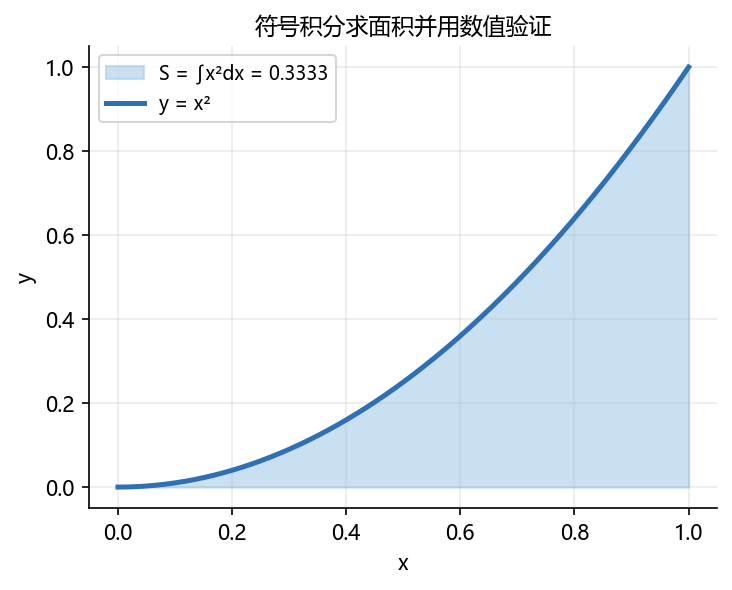
\includegraphics[keepaspectratio,alt={符号积分求面积}]{figures/02-sympy/sympy_area.png}}
\caption{符号积分求面积}
\end{figure}

\subsubsection{分析}\label{ux5206ux6790-2}

\begin{itemize}
\tightlist
\item
  SymPy 给出精确的 \(1/3\)，而 NumPy 的
  \texttt{np.trapz}/数值积分只能给出近似；
\item
  \texttt{sp.N(area)} 输出
  0.333333333333333，说明符号结果与数值结果一致；
\item
  这正体现``先符号推导得到公式，再数值计算/可视化''的方法论。
\end{itemize}

\subsubsection{拓展任务}\label{ux62d3ux5c55ux4efbux52a1-2}

\begin{enumerate}
\def\labelenumi{\arabic{enumi}.}
\tightlist
\item
  改求 \(y=e^{-x}\) 在 \([0,1]\) 上的面积，并与
  \texttt{scipy.integrate.quad} 比较；
\item
  求曲线 \(y=x^2\) 绕 \(x\)
  轴旋转一周的旋转体体积：\(\pi\int_0^1 x^4 dx\)，用 SymPy 验证；
\item
  把 \([0,1]\) 换成 \([a,b]\) 符号区间，观察 SymPy 是否保留符号结果。
\end{enumerate}

\begin{center}\rule{0.5\linewidth}{0.5pt}\end{center}

\subsection{案例 2：符号导数 → 切线方程 →
数值验证}\label{ux6848ux4f8b-2ux7b26ux53f7ux5bfcux6570-ux5207ux7ebfux65b9ux7a0b-ux6570ux503cux9a8cux8bc1}

\subsubsection{背景}\label{ux80ccux666f-3}

求 \(y=\sin x\) 在 \(x=1\) 处的切线方程。先用 SymPy 求导得到
\(\cos x\)，再求斜率 \(\cos(1)\)，最后用 \texttt{lambdify}
画图，并与数值差商验证。

\subsubsection{代码}\label{ux4ee3ux7801-2}

\begin{Shaded}
\begin{Highlighting}[]
\ImportTok{import}\NormalTok{ sympy }\ImportTok{as}\NormalTok{ sp}
\ImportTok{import}\NormalTok{ numpy }\ImportTok{as}\NormalTok{ np}
\NormalTok{x }\OperatorTok{=}\NormalTok{ sp.symbols(}\StringTok{\textquotesingle{}x\textquotesingle{}}\NormalTok{)}
\NormalTok{f }\OperatorTok{=}\NormalTok{ sp.sin(x)}
\NormalTok{df }\OperatorTok{=}\NormalTok{ sp.diff(f, x)}
\BuiltInTok{print}\NormalTok{(df)   }\CommentTok{\# cos(x)}

\NormalTok{a }\OperatorTok{=} \DecValTok{1}
\NormalTok{slope }\OperatorTok{=}\NormalTok{ sp.N(df.subs(x, a))}
\BuiltInTok{print}\NormalTok{(slope)   }\CommentTok{\# cos(1) ≈ 0.540302305868140}

\NormalTok{tangent }\OperatorTok{=}\NormalTok{ sp.simplify(df.subs(x, a) }\OperatorTok{*}\NormalTok{ (x }\OperatorTok{{-}}\NormalTok{ a) }\OperatorTok{+}\NormalTok{ f.subs(x, a))}
\BuiltInTok{print}\NormalTok{(tangent)}

\CommentTok{\#\# 数值差商验证导数}
\NormalTok{h }\OperatorTok{=} \FloatTok{1e{-}6}
\NormalTok{numeric\_deriv }\OperatorTok{=}\NormalTok{ (sp.sin(a }\OperatorTok{+}\NormalTok{ h) }\OperatorTok{{-}}\NormalTok{ sp.sin(a }\OperatorTok{{-}}\NormalTok{ h)) }\OperatorTok{/}\NormalTok{ (}\DecValTok{2}\OperatorTok{*}\NormalTok{h)}
\BuiltInTok{print}\NormalTok{(}\BuiltInTok{float}\NormalTok{(sp.N(numeric\_deriv)))}
\end{Highlighting}
\end{Shaded}

\begin{Shaded}
\begin{Highlighting}[]
\NormalTok{cos(x)}
\NormalTok{0.540302305868140}
\NormalTok{(x {-} 1)*cos(1) + sin(1)}
\NormalTok{0.540302305840346}
\end{Highlighting}
\end{Shaded}

\subsubsection{可视化}\label{ux53efux89c6ux5316-1}

\begin{Shaded}
\begin{Highlighting}[]
\ImportTok{import}\NormalTok{ matplotlib.pyplot }\ImportTok{as}\NormalTok{ plt}

\NormalTok{plt.rcParams[}\StringTok{\textquotesingle{}font.sans{-}serif\textquotesingle{}}\NormalTok{] }\OperatorTok{=}\NormalTok{ [}\StringTok{\textquotesingle{}Microsoft YaHei\textquotesingle{}}\NormalTok{, }\StringTok{\textquotesingle{}SimHei\textquotesingle{}}\NormalTok{, }\StringTok{\textquotesingle{}DejaVu Sans\textquotesingle{}}\NormalTok{]}
\NormalTok{plt.rcParams[}\StringTok{\textquotesingle{}axes.unicode\_minus\textquotesingle{}}\NormalTok{] }\OperatorTok{=} \VariableTok{False}

\KeywordTok{def}\NormalTok{ tangent\_num(v):}
    \ControlFlowTok{return} \BuiltInTok{float}\NormalTok{(sp.N(tangent.subs(x, v)))}

\NormalTok{xn }\OperatorTok{=}\NormalTok{ np.linspace(}\OperatorTok{{-}}\DecValTok{1}\NormalTok{, }\DecValTok{3}\NormalTok{, }\DecValTok{400}\NormalTok{)}
\NormalTok{plt.figure(figsize}\OperatorTok{=}\NormalTok{(}\FloatTok{5.8}\NormalTok{, }\FloatTok{4.0}\NormalTok{))}
\NormalTok{plt.plot(xn, np.sin(xn), color}\OperatorTok{=}\StringTok{\textquotesingle{}\#2f6fb3\textquotesingle{}}\NormalTok{, lw}\OperatorTok{=}\FloatTok{2.4}\NormalTok{, label}\OperatorTok{=}\StringTok{\textquotesingle{}y = sin(x)\textquotesingle{}}\NormalTok{)}
\NormalTok{plt.plot(xn, [tangent\_num(v) }\ControlFlowTok{for}\NormalTok{ v }\KeywordTok{in}\NormalTok{ xn], color}\OperatorTok{=}\StringTok{\textquotesingle{}\#e07b39\textquotesingle{}}\NormalTok{, lw}\OperatorTok{=}\DecValTok{2}\NormalTok{, ls}\OperatorTok{=}\StringTok{\textquotesingle{}{-}{-}\textquotesingle{}}\NormalTok{,}
\NormalTok{         label}\OperatorTok{=}\SpecialStringTok{f\textquotesingle{}切线 (斜率 ≈ }\SpecialCharTok{\{}\BuiltInTok{float}\NormalTok{(slope)}\SpecialCharTok{:.4f\}}\SpecialStringTok{)\textquotesingle{}}\NormalTok{)}
\NormalTok{plt.plot([a], [np.sin(a)], }\StringTok{\textquotesingle{}o\textquotesingle{}}\NormalTok{, color}\OperatorTok{=}\StringTok{\textquotesingle{}\#c0392b\textquotesingle{}}\NormalTok{, ms}\OperatorTok{=}\DecValTok{7}\NormalTok{, label}\OperatorTok{=}\SpecialStringTok{f\textquotesingle{}切点 x=}\SpecialCharTok{\{}\NormalTok{a}\SpecialCharTok{\}}\SpecialStringTok{\textquotesingle{}}\NormalTok{)}
\NormalTok{plt.axhline(}\DecValTok{0}\NormalTok{, color}\OperatorTok{=}\StringTok{\textquotesingle{}\#666\textquotesingle{}}\NormalTok{, lw}\OperatorTok{=}\FloatTok{0.7}\NormalTok{)}\OperatorTok{;}\NormalTok{ plt.axvline(}\DecValTok{0}\NormalTok{, color}\OperatorTok{=}\StringTok{\textquotesingle{}\#666\textquotesingle{}}\NormalTok{, lw}\OperatorTok{=}\FloatTok{0.7}\NormalTok{)}
\NormalTok{plt.xlabel(}\StringTok{\textquotesingle{}x\textquotesingle{}}\NormalTok{)}\OperatorTok{;}\NormalTok{ plt.ylabel(}\StringTok{\textquotesingle{}y\textquotesingle{}}\NormalTok{)}
\NormalTok{plt.title(}\StringTok{\textquotesingle{}符号导数 → 切线方程\textquotesingle{}}\NormalTok{, fontsize}\OperatorTok{=}\DecValTok{11}\NormalTok{)}
\NormalTok{plt.legend()}\OperatorTok{;}\NormalTok{ plt.grid(alpha}\OperatorTok{=}\FloatTok{0.25}\NormalTok{)}
\NormalTok{plt.savefig(}\StringTok{\textquotesingle{}figures/02{-}sympy/sympy\_tangent.png\textquotesingle{}}\NormalTok{, bbox\_inches}\OperatorTok{=}\StringTok{\textquotesingle{}tight\textquotesingle{}}\NormalTok{)}
\NormalTok{plt.show()}
\end{Highlighting}
\end{Shaded}

\begin{figure}
\centering
\pandocbounded{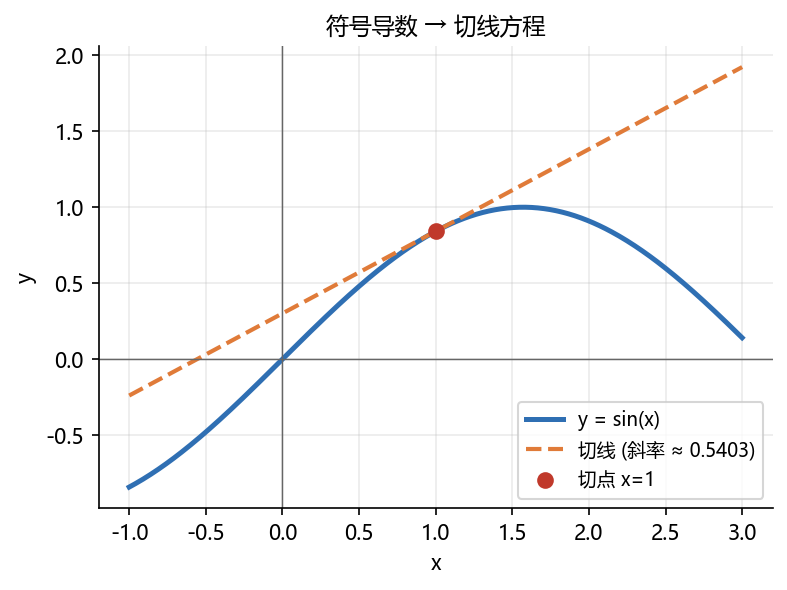
\includegraphics[keepaspectratio,alt={符号导数与切线}]{figures/02-sympy/sympy_tangent.png}}
\caption{符号导数与切线}
\end{figure}

\subsubsection{分析}\label{ux5206ux6790-3}

\begin{itemize}
\tightlist
\item
  符号求导得到 \(\cos x\)，代入 \(x=1\) 得斜率 ≈ 0.5403；
\item
  数值中心差商（\(h=10^{-6}\)）与符号导数一致，说明推导正确；
\item
  切线方程被 \texttt{simplify} 整理成
  \texttt{(x-1)*cos(1)\ +\ sin(1)}，可直接用于绘图/插值。
\end{itemize}

\subsubsection{拓展任务}\label{ux62d3ux5c55ux4efbux52a1-3}

\begin{enumerate}
\def\labelenumi{\arabic{enumi}.}
\tightlist
\item
  用 \texttt{lambdify} 把 \texttt{tangent} 和 \texttt{f}
  都转成数值函数，再比较在 \(x=0.5,1,1.5\) 处的数值；
\item
  求 \(y=\ln(x)\) 在 \(x=2\) 的法线方程并绘图；
\item
  把切线推广到二元函数（用梯度向量/切平面概念）。
\end{enumerate}

\begin{center}\rule{0.5\linewidth}{0.5pt}\end{center}

\subsection{案例
3：解方程并把根画在数轴上}\label{ux6848ux4f8b-3ux89e3ux65b9ux7a0bux5e76ux628aux6839ux753bux5728ux6570ux8f74ux4e0a}

\subsubsection{背景}\label{ux80ccux666f-4}

用 \texttt{solve} 求出多项式 \(x^2-5x+4=0\)
的根，并把函数曲线与根标注在同一张图上，直观理解``方程的解''就是``函数与
\(x\) 轴交点''。

\subsubsection{代码与输出}\label{ux4ee3ux7801ux4e0eux8f93ux51fa}

\begin{Shaded}
\begin{Highlighting}[]
\ImportTok{import}\NormalTok{ sympy }\ImportTok{as}\NormalTok{ sp}
\NormalTok{x }\OperatorTok{=}\NormalTok{ sp.symbols(}\StringTok{\textquotesingle{}x\textquotesingle{}}\NormalTok{)}
\NormalTok{p }\OperatorTok{=}\NormalTok{ x}\OperatorTok{**}\DecValTok{2} \OperatorTok{{-}} \DecValTok{5}\OperatorTok{*}\NormalTok{x }\OperatorTok{+} \DecValTok{4}
\NormalTok{roots }\OperatorTok{=} \BuiltInTok{sorted}\NormalTok{(sp.solve(p, x))}
\BuiltInTok{print}\NormalTok{(roots)}
\BuiltInTok{print}\NormalTok{([}\BuiltInTok{float}\NormalTok{(sp.N(r)) }\ControlFlowTok{for}\NormalTok{ r }\KeywordTok{in}\NormalTok{ roots])}
\end{Highlighting}
\end{Shaded}

\begin{Shaded}
\begin{Highlighting}[]
\NormalTok{[1, 4]}
\NormalTok{[1.0, 4.0]}
\end{Highlighting}
\end{Shaded}

\begin{figure}
\centering
\pandocbounded{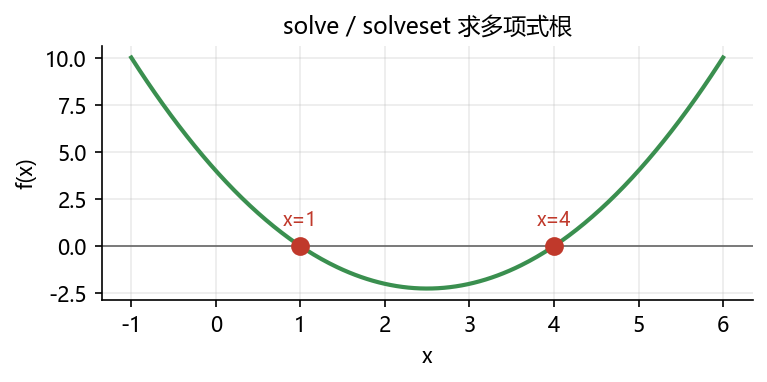
\includegraphics[keepaspectratio,alt={多项式根可视化}]{figures/02-sympy/sympy_roots.png}}
\caption{多项式根可视化}
\end{figure}

\subsubsection{分析}\label{ux5206ux6790-4}

\begin{itemize}
\tightlist
\item
  \texttt{solve} 精确返回整数根 1 和 4，无需浮点迭代；
\item
  根的位置与曲线穿越 \(x\)
  轴的位置一致，图片直观地体现``解方程=找零点''。
\end{itemize}

\subsubsection{拓展任务}\label{ux62d3ux5c55ux4efbux52a1-4}

\begin{enumerate}
\def\labelenumi{\arabic{enumi}.}
\tightlist
\item
  改求 \(x^3-6x^2+11x-6=0\) 的三个根并画图；
\item
  用 \texttt{solveset(...,\ domain=sp.S.Complexes)} 求解
  \(x^2+1=0\)，解释为什么实数域为空；
\item
  用 \texttt{lambdify} 把 \texttt{p} 转成数值函数，用 \texttt{np.roots}
  验证数值根。
\end{enumerate}

\subsection{本章综合练习（上机任务）}\label{ux672cux7ae0ux7efcux5408ux7ec3ux4e60ux4e0aux673aux4efbux52a1-1}

\begin{enumerate}
\def\labelenumi{\arabic{enumi}.}
\tightlist
\item
  用 SymPy 推导 \(y=\sqrt{x}\) 在 \([0,4]\) 上的面积，用 matplotlib
  绘制填充区域并标注精确值；
\item
  求 \(f(x)=x^3-3x\) 的极值点（提示：令 \(f'(x)=0\) 用
  \texttt{solve}），并画函数与极值点图；
\item
  把案例 1--3 整理成一个 \texttt{.ipynb}，写一份 200
  字以内的结论，说明``符号解 vs 数值解''各自的优势。
\end{enumerate}

\subsection{延伸阅读}\label{ux5ef6ux4f38ux9605ux8bfb-8}

\begin{itemize}
\tightlist
\item
  SymPy
  官方绘图（Plotting）模块：https://docs.sympy.org/latest/modules/plotting.html
\item
  Matplotlib
  填充区域：https://matplotlib.org/stable/api/\_as\_gen/matplotlib.pyplot.fill\_between.html
\item
  NumPy
  数值求根（np.roots）：https://numpy.org/doc/stable/reference/generated/numpy.roots.html
\end{itemize}

\section{04
常见误区与技巧}\label{ux5e38ux89c1ux8befux533aux4e0eux6280ux5de7-1}

\begin{quote}
本章为新增``查漏补缺''页：把学生最容易踩的坑集中列出，并给出正确的写法和性能技巧。
\end{quote}

\subsection{1.
高频误区速查表}\label{ux9ad8ux9891ux8befux533aux901fux67e5ux8868-1}

{\def\LTcaptype{none} % do not increment counter
\begin{longtable}[]{@{}
  >{\raggedright\arraybackslash}p{(\linewidth - 6\tabcolsep) * \real{0.2500}}
  >{\raggedright\arraybackslash}p{(\linewidth - 6\tabcolsep) * \real{0.2500}}
  >{\raggedright\arraybackslash}p{(\linewidth - 6\tabcolsep) * \real{0.2500}}
  >{\raggedright\arraybackslash}p{(\linewidth - 6\tabcolsep) * \real{0.2500}}@{}}
\toprule\noalign{}
\begin{minipage}[b]{\linewidth}\raggedright
\#
\end{minipage} & \begin{minipage}[b]{\linewidth}\raggedright
误区 / 错误写法
\end{minipage} & \begin{minipage}[b]{\linewidth}\raggedright
正确做法
\end{minipage} & \begin{minipage}[b]{\linewidth}\raggedright
原因
\end{minipage} \\
\midrule\noalign{}
\endhead
\bottomrule\noalign{}
\endlastfoot
1 & \texttt{pi\ =\ 3.14159} 然后参与符号运算 & 用 \texttt{sp.pi}（符号
π） & 浮点近似破坏精确性 \\
2 & \texttt{x\ +\ y\ ==\ y\ +\ x} 判断表达式相等 &
\texttt{sp.simplify((x+y)\ -\ (y+x))\ ==\ 0} 或
\texttt{(x+y).equals(y+x)} & \texttt{==} 比较的是结构不是数学等价 \\
3 & \texttt{sp.sqrt(x**2)} 期望得到 \texttt{x} &
\texttt{x\ =\ sp.Symbol(\textquotesingle{}x\textquotesingle{},\ positive=True)}
& 若无假设，\texttt{sqrt(x**2)=\textbar{}x\textbar{}} 更严谨 \\
4 & 用 \texttt{math.sin(x)} 而 \texttt{x} 是符号 & 用 \texttt{sp.sin(x)}
& \texttt{math} 只能处理浮点数 \\
5 & 以为 \texttt{lambdify} 返回符号表达式 &
它是数值函数，输入输出都是数值/数组 & 符号→数值的桥梁，不可再
\texttt{diff} \\
6 & \texttt{A\ *\ B} 想要 NumPy 式的逐元素乘 & SymPy \texttt{Matrix} 的
\texttt{*} 是矩阵乘；逐元素需 \texttt{sp.Matrix(A.applyfunc)} &
两种库的语义不同 \\
7 & \texttt{sp.solve(eq,\ x)} 忘记 \texttt{Eq} & 可以写
\texttt{sp.solve(eq,\ x)}（eq 视为=0）或
\texttt{sp.solve(sp.Eq(f,\ 0),\ x)} & 传入非 Eq 表达式默认等于 0 \\
8 & 用 \texttt{dsolve(eq)} 但没定义 \texttt{Function} &
\texttt{y\ =\ sp.Function(\textquotesingle{}y\textquotesingle{})(x)}；初值用
\texttt{ics=\{y.subs(x,0):\ 1\}} & 未定义函数会让 dsolve
报错/无法识别 \\
9 & 期望 \texttt{simplify} 万能 & 配合
\texttt{trigsimp}、\texttt{together}、\texttt{cancel}、\texttt{radsimp}
& 化简是启发式的 \\
10 & 用 \texttt{solve} 求所有复数根当实数用 & 用
\texttt{solveset(...,\ domain=sp.S.Reals)} 或 \texttt{real\_roots} &
不同求解函数返回集不同 \\
\end{longtable}
}

\subsection{2. 原理级难点：符号 vs
数值}\label{ux539fux7406ux7ea7ux96beux70b9ux7b26ux53f7-vs-ux6570ux503c}

\begin{Shaded}
\begin{Highlighting}[]
\ImportTok{import}\NormalTok{ sympy }\ImportTok{as}\NormalTok{ sp}
\NormalTok{x }\OperatorTok{=}\NormalTok{ sp.Symbol(}\StringTok{\textquotesingle{}x\textquotesingle{}}\NormalTok{)}
\NormalTok{expr }\OperatorTok{=}\NormalTok{ x}\OperatorTok{**}\DecValTok{2} \OperatorTok{+} \DecValTok{1}          \CommentTok{\# 符号表达式}
\BuiltInTok{print}\NormalTok{(}\BuiltInTok{type}\NormalTok{(expr))        }\CommentTok{\# \textless{}class \textquotesingle{}sympy.core.add.Add\textquotesingle{}\textgreater{}}

\NormalTok{val }\OperatorTok{=}\NormalTok{ expr.subs(x, }\DecValTok{2}\NormalTok{)    }\CommentTok{\# 仍是符号（整数 5）}
\BuiltInTok{print}\NormalTok{(val, }\BuiltInTok{type}\NormalTok{(val))}

\NormalTok{num }\OperatorTok{=}\NormalTok{ sp.N(expr.subs(x, }\DecValTok{2}\NormalTok{))   }\CommentTok{\# 数值}
\BuiltInTok{print}\NormalTok{(num, }\BuiltInTok{type}\NormalTok{(num))}

\NormalTok{f }\OperatorTok{=}\NormalTok{ sp.lambdify(x, expr, }\StringTok{\textquotesingle{}numpy\textquotesingle{}}\NormalTok{)}
\BuiltInTok{print}\NormalTok{(f(}\DecValTok{2}\NormalTok{))              }\CommentTok{\# 数值 5}
\end{Highlighting}
\end{Shaded}

要点：\textbf{符号对象}不参与浮点运算，只有
\texttt{subs}+\texttt{N}/\texttt{evalf} 或 \texttt{lambdify}
才会产生数值结果。

\subsection{3.
求解函数的选型}\label{ux6c42ux89e3ux51fdux6570ux7684ux9009ux578b}

{\def\LTcaptype{none} % do not increment counter
\begin{longtable}[]{@{}lll@{}}
\toprule\noalign{}
场景 & 推荐函数 & 说明 \\
\midrule\noalign{}
\endhead
\bottomrule\noalign{}
\endlastfoot
一元方程 & \texttt{solve} / \texttt{solveset} & \texttt{solveset}
更严谨 \\
线性方程组 & \texttt{linsolve} & 可传方程列表或 \texttt{(A,\ b)} \\
非线性方程组 & \texttt{nonlinsolve} / \texttt{solve} &
结果可能含复数解 \\
初等矩阵运算 & \texttt{Matrix} + 方法 &
\texttt{det}、\texttt{inv}、\texttt{eigenvals} \\
符号→数值 & \texttt{lambdify} & 指定
\texttt{\textquotesingle{}numpy\textquotesingle{}} \\
\end{longtable}
}

\subsection{4. 性能技巧}\label{ux6027ux80fdux6280ux5de7-1}

\begin{itemize}
\item
  \textbf{优先 \texttt{lambdify} 而不是逐点
  \texttt{subs}/\texttt{evalf}}：对大量数值点，先转成 NumPy
  函数再向量化计算，速度可提升百倍：

\begin{Shaded}
\begin{Highlighting}[]
\ImportTok{import}\NormalTok{ sympy }\ImportTok{as}\NormalTok{ sp, numpy }\ImportTok{as}\NormalTok{ np}
\NormalTok{x }\OperatorTok{=}\NormalTok{ sp.symbols(}\StringTok{\textquotesingle{}x\textquotesingle{}}\NormalTok{)}
\NormalTok{f }\OperatorTok{=}\NormalTok{ sp.lambdify(x, sp.sin(x)}\OperatorTok{/}\NormalTok{x, }\StringTok{\textquotesingle{}numpy\textquotesingle{}}\NormalTok{)}
\NormalTok{xs }\OperatorTok{=}\NormalTok{ np.linspace(}\FloatTok{0.001}\NormalTok{, }\DecValTok{10}\NormalTok{, }\DecValTok{100000}\NormalTok{)}
\NormalTok{ys }\OperatorTok{=}\NormalTok{ f(xs)          }\CommentTok{\# 一次向量化，比循环快得多}
\end{Highlighting}
\end{Shaded}
\item
  \textbf{\texttt{simplify} 要慎用}：可能很慢、甚至把结果变得更长；先试
  \texttt{cancel}/\texttt{together}/\texttt{trigsimp}；
\item
  \textbf{避免反复重建符号}：把符号与常用表达式定义一次，不要在循环里重复
  \texttt{symbols}；
\item
  \textbf{大矩阵用 \texttt{sp.Matrix} 的数值化}：若最终只需数值，考虑
  \texttt{sp.Matrix(...).evalf()} 或转成 NumPy \texttt{np.array(...)}
  再算；
\item
  \textbf{\texttt{nsimplify}
  做``反向''精确化}：把浮点近似还原为有理数/根式（如
  \texttt{sp.nsimplify(0.333333)} → \texttt{1/3}）。
\end{itemize}

\subsection{5. 调试建议}\label{ux8c03ux8bd5ux5efaux8bae-1}

\begin{enumerate}
\def\labelenumi{\arabic{enumi}.}
\tightlist
\item
  打印 \texttt{type(expr)}：确认是符号还是数值；
\item
  用 \texttt{sp.srepr(expr)} 查看底层树状结构，定位``为什么没化简''；
\item
  \texttt{expr.free\_symbols} 查看表达式含哪些符号；
\item
  \texttt{sp.solve} 无解时先试 \texttt{solveset}，再看 \texttt{domain}；
\item
  符号求导/积分结果可疑时，用数值验证：\texttt{sp.N(expr.subs(x,\ a))}
  与手工/数值结果对比；
\item
  复杂方程先 \texttt{sp.simplify} 或 \texttt{sp.expand} 再求。
\end{enumerate}

\subsection{6.
本章小结（自测）}\label{ux672cux7ae0ux5c0fux7ed3ux81eaux6d4b-1}

\begin{itemize}
\tightlist
\item[$\square$]
  能说明 \texttt{symbols} 与 \texttt{Symbol} 的区别；
\item[$\square$]
  能区分符号 π 与 \texttt{math.pi}；
\item[$\square$]
  能正确判断两个符号表达式是否数学等价；
\item[$\square$]
  能求极限、导数、积分并用数值验证；
\item[$\square$]
  能用
  \texttt{solve}/\texttt{solveset}/\texttt{linsolve}/\texttt{nonlinsolve}
  解对应问题；
\item[$\square$]
  会用 \texttt{lambdify} 把表达式转成数值函数；
\item[$\square$]
  会用 \texttt{dsolve} 解一/二阶微分方程并给定初值；
\item[$\square$]
  能用 \texttt{Matrix} 求特征值、雅可比矩阵。
\end{itemize}

\subsection{延伸阅读}\label{ux5ef6ux4f38ux9605ux8bfb-9}

\begin{itemize}
\tightlist
\item
  SymPy 官方 Tutorial：https://docs.sympy.org/latest/tutorial/index.html
\item
  SymPy 官方 FAQ：https://docs.sympy.org/latest/tutorial/gotchas.html
\item
  SymPy
  官方性能/数值化建议：https://docs.sympy.org/latest/modules/utilities/lambdify.html
\end{itemize}

\newpage
